\ofsubsection{Gold Saucer}
%
%
%
%It's our most popular employee, Mr. Hangman. - receptionist
%
%Just think of 'GP' as money that you can only use at the Gold Saucer.
%I wish we could just forget everything and have fun! -aerith
%
% 
%
\ofquote{"Welcome to Gold Saucer! You will be moved and excited, thrilled and terrified! Led from one zone to another... unlike anything you've ever experienced! Make your memories... today."}{Advertisement}
%
\begin{center} 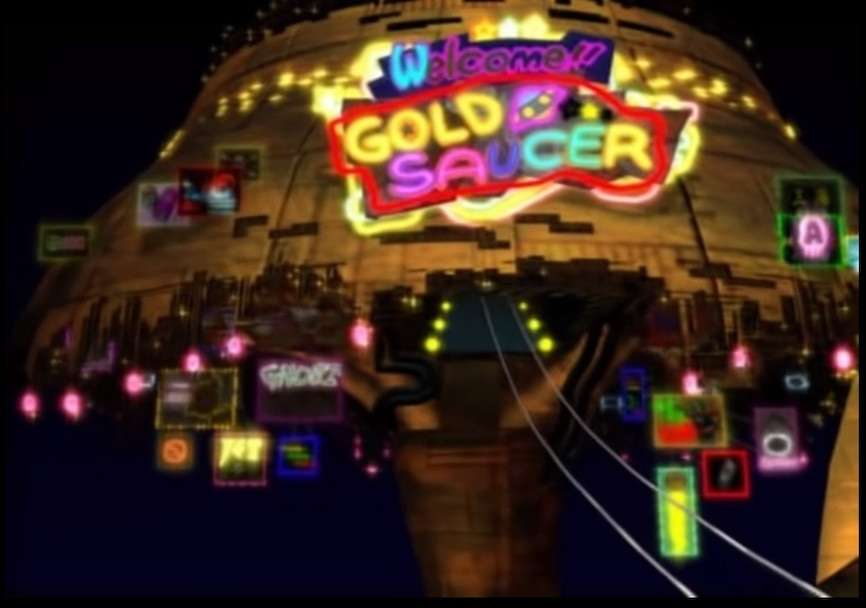
\includegraphics[width=\columnwidth]{./art/goldsaucer/goldsaucer.jpg} \end{center}
%
\vfill
%
\accf{Gold Saucer} is an amusement park with a wide variety of games and attractions for the player characters to enjoy and compete in.
You can either use the entire park as a location in your game world or just pick out attractions that you are particularly interested in.
As such, the following content is mostly a list of park attractions with their respective rules.
Gold Saucer is built as high tower surrounded by multiple large structures that contain the different attractions.
The park's entrance can only be reached with a cable car, the entry fee of 50G per person includes the fare.
Alternatively, players can also buy a lifetime pass for 500G.
Also, taking part in an attraction usually costs an amount of Gold Points (GP), which is the only valid currency inside the park.
GP can be bought and sold at the park's entrance at a rate of 1 GP per 50G.
Right behind the entrance, the players find themselves in a central hub, from which they can move between the major locations of the park through a series of tubes.
%
\vfill
%
\begin{center} 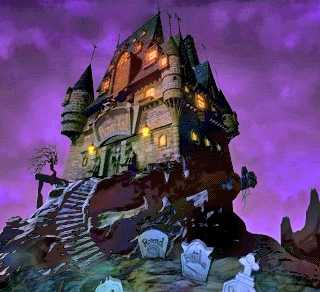
\includegraphics[width=\columnwidth]{./art/goldsaucer/hauntedhouse.jpg} \end{center}
%
\newpage
%
This document primarily focuses on the major attractions of the park and offers detailed rules for recreating them in your game.
In contrast, there are also many minor attractions of Gold Saucer, some of which are listed below: \ofrow
\ofbullet{\accf{Fortune Teller:} a strange being that looks like a big plush toy with a cat sitting on top of it. It offers a fortune telling to the party for the cost of 2 GP, a service which they can only use once. The GM should ensure that the teller gives the party an accurate prediction or a useful advice for the future.}
\ofbullet{\accf{Gondola:} for a price of 1 GP per person, the party can take a ride on a big gondala, which allows them to catch a nice view of the whole park at its zenith. If the players enter the gondola at midnight, they can also observe the daily fireworks of Gold Saucer. The perfect spot for a date!}
\ofbullet{\accf{Haunted House:} a creepy castle that has been prepared to scare its visitors through the placement of fake props such as ghosts, skelletons and spiders. Upon entering the first time, every player has to perform a DC~8 check and upon failure he becomes scared or creeped out. The haunted house acts as a hotel, the party can spend the night here for a price of 1 GP per person.}
%
\\\\
%
%\ofquote{"What you pursue will be yours. But you will lose something dear."}{Fortune Teller}\\\\
\ofquote{"While your ride's going ZOOM, you're going BANG BANG, and things are going PHEW PHEW and you destroy them with a big BOOM. Pretty simple, isn't it?"\\}{Employee}
%
%
%
%
%
%
\begin{center} 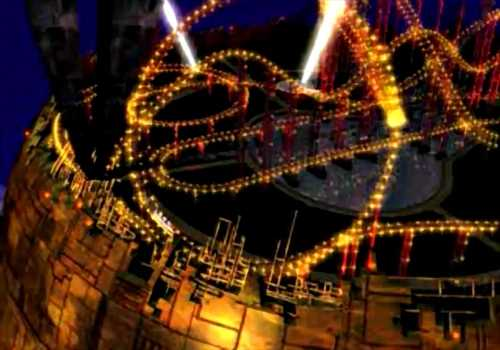
\includegraphics[width=\columnwidth]{./art/goldsaucer/shootingcoaster.jpg} \end{center}
The \accf{Shooting Coaster} is a roller coaster game with an entry fee of 1 GP per person.
Each seat has a turret built in that visitors can use to shoot various projections that appear throughout the coaster ride.
Hitting a projected object grants players an amount of points and they receive prizes for reaching a high score.
The duration of the ride is split into 5 rounds. 
At the start of each round, the GM rolls an amount of dice equal to the party size plus 1 to determine which projections appear in this round. 
During each round, each player takes a turn in which they can try to shoot one of the projections of their choice.
To do so they have to pass a check, the DC depends on the type of the projection as some are faster and smaller and thus harder to hit than others. 
However, projections that are harder to hit also grant more points.
Characters that can use Bows or Guns or have other experiences with ranged weapons, gain Advantage on this check.
Projections disappear either after they are successfully hit or at the end of a round.
The table below shows all possible projections, the die number (Nr.) at which they appear, the DC required to hit them and the amount of points granted when done so.
%
\\\\
%
\oftable{p{0.2\columnwidth} p{0.3\columnwidth} p{0.2\columnwidth} r}
{\accf{Nr.} & \accf{Name} & \accf{DC} & \accf{Points}}
{
	1 & Cactus 	& 5  & 10 \ofrow
	2 & Balloon & 6  & 15 \ofrow		
	3 & Plane   & 7  & 20 \ofrow
	4 & Ghost 	& 8  & 30 \ofrow
	5 & Star 	& 9  & 50 \ofrow
	6 & UFO   	& 10 & 70 \ofrow			
}
%
\\\\
%
During the ride, each player should keep track of the amount of points they have scored and after the 5th round is completed, every participant receives the following prize based on his or her score.
%
\\\\
%
\oftable{p{0.5\columnwidth} p{0.5\columnwidth}}
{\accf{Score} & \accf{Prize}}
{
	less than 25 & Potion \ofrow
	25 to 50 & DEF Plus \ofrow
	50 to 75 & X-Potion \ofrow		
	75 to 100 & Moogle Charm \ofrow
	more than 100 & Ribbon  																				
}
%
\\\\
%
%
%
%
%
\begin{center} 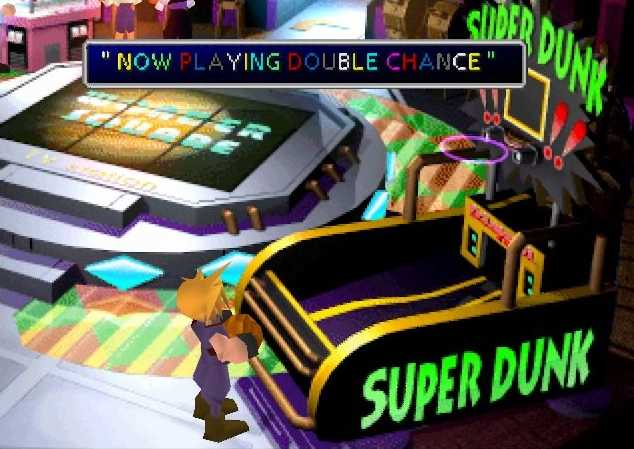
\includegraphics[width=\columnwidth]{./art/goldsaucer/superdunk.jpg} \end{center}
\accf{Super Dunk} is a basketball game that costs 2 GP per player to play. 
All participants stand in a dedicated spot in front of the machine and balls are given out to the players who have to successfully throw it into the hoops.
The game is played round by round, and in each one, every participant performs a throw.
A DC~6 check decides whether a throw is successful, characters with especially good coordination gain Advantage on this check.
For each successful consecutive throw, a player's prize amount is increased by 1 GP.
A player that misses a shot is immediately eliminated from the game at which point his accumulated prize amount is paid out.
After every 3 successful rounds the players receive a Double Chance, at which point they can decide to stop and collect their prize or continue throwing.
In the latter case, a player's current prize amount is doubled if he succeeds the next throw, but if he fails, he is eliminated and receives no prize.
%
\vfill
%
\ofquote{"I wish we could just forget everything and have fun!"\\}{Aerith}
%
\vfill
%
%
%
%
\begin{center} 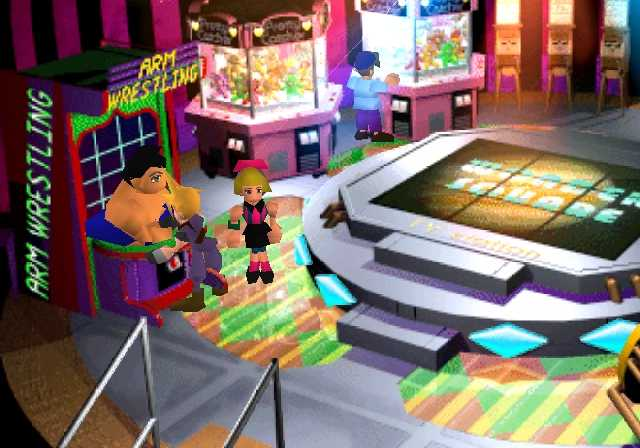
\includegraphics[width=\columnwidth]{./art/goldsaucer/armwrestling.jpg} \end{center}
\accf{Arm Wrestling} is a strength competition that costs 1 GP to participate in.
The game is played by a single player who faces up to three champions, one after the other, in an arm wrestling match.
The state of a match is tracked as a scale from +3 to -3, the player wins when it reaches +3 and the opponent wins when it reaches -3.
This score is meant to represent the angle of the competitors' arms and it starts at 0.
The player and the GM who plays as the champion, make opposed checks until one side wins the match.
On each check, the score increases by 1 if the player has a higher result and it is reduced 1 if the champion has a higher roll.
Players with particularly high strength or athletic ability gain Advantage on this check and the champions gain a flat bonus due to their experience in the sport.
After defeating a champion, the total prize amount is increased and the player can decide to either stop and collect it or to challenge the next stronger champion.
In the latter case, the player gains no prize if he loses the match.
The table below lists all champions, the bonus they gain on the checks and the prizes for defeating them.
%
\\\\
%
\oftable{p{0.35\columnwidth} p{0.3\columnwidth} p{0.2\columnwidth}}
{\accf{Champion} & \accf{Bonus} & \accf{Prize}}
{
	Body Builder & +1 & 2 GP \ofrow
	Sumo 		 & +2 & 5 GP \ofrow
	Wrestler 	 & +3 & 10 GP \ofrow
}
%
\clearpage
%
%
%
%
%
%
%
%
\begin{center} 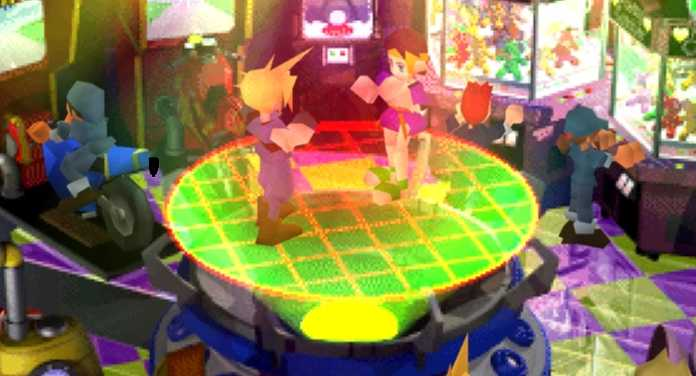
\includegraphics[width=\columnwidth]{./art/goldsaucer/battler.jpg} \end{center}
\accf{Battler} is a fighting game that costs 1 GP to play.
The game is played by a single who faces up to four fighters, one by one, that are played by the GM.
A match is played out in multiple rounds and in each round, the combatants can choose one of 3 actions: 
low attack (LA), middle attack (MA) and high attack (HA).
The player can freely decide which action to take and then the GM rolls 1d to determine the action taken by the opponent.
HA beats LA, MA beats HA, LA beats MA and if both take the same action they just cancel each other out.
The winner of a round gains 1 point and the first one to have 3 points wins the match.
After defeating a fighter, the total prize amount is increased and the player can decide to either stop and collect it or to challenge the next stronger fighter.
In the latter case, the player gains no prize if he loses the match.
The table below shows all fighters, which actions they take depending on the result of your rolls and the prizes for defeating them.
%
\\\\
%
\oftable{p{0.22\columnwidth} p{0.5\columnwidth} p{0.15\columnwidth}}
{\accf{Fighter} & \accf{Actions} & \accf{Prize}}
{
	Zell 	& 1-4: LA, 5-6: HA & 2 GP \ofrow
	Sabin	& 1: LA, 3-5: MA, 6: HA & 5 GP \ofrow
	Tifa 	& 1-2: LA, 3-4: MA, 5-6: HA & 10 GP \ofrow
}
%
\vfill
%
\ofquote{"Almost... Crap! No cigar... You sure do need a lot of money here. Please, don't talk to me right now. I get so caught up in these."}{Visitor}
%
\vfill
%
%
%
%
%
%
\
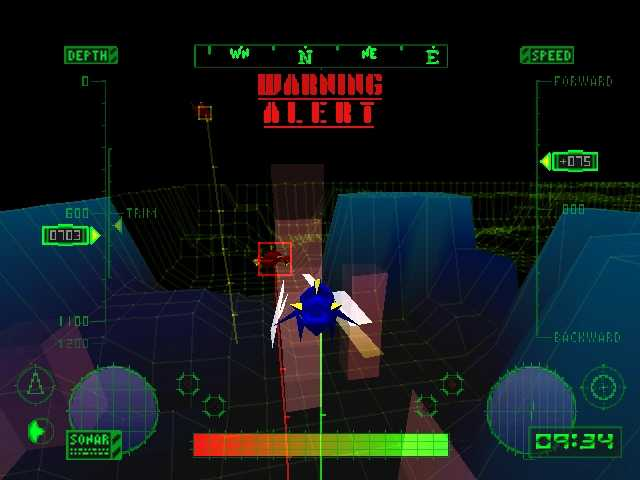
\includegraphics[width=\columnwidth]{./art/goldsaucer/submarine.jpg}
%
\newpage
%
\accf{Torpedo Attack} is a submarine battle game that costs 2 GP to play. 
The game can be played by up to 3 players who can split the 3 possible submarine actions between them.
Torpedo Attack is similar to combat and the players have to defeat all enemy submarines while making sure theirs stays intact. 
A match is played out in multiple rounds and in each round, the player submarine can take 2 of the following 3 actions: \\
\ofbullet{\accf{Move:} roll 1d. The result times 10 is the amount of units you can move in this round.}\\
\ofbullet{\accf{Shoot:} choose an enemy submarine within 30u. Make a DC~7 check, if you succeed, the enemy submarine is destroyed.}\\
\ofbullet{\accf{Sonar:} make a DC~7 check, if you succeed, all mines within 50u are revealed.}\\
Enemy submarines take their actions right after the players, they can shoot in the same manner and move a distance of up to 30u, but they are not affected by mines.
The player submarine can survive up to 3 damage, getting hit by an enemy shot or moving over a mine causes 1 damage.
Use a map similar to the one below to visualize the game.
%
\vfill
%
\begin{figure}[h]
	\centering
	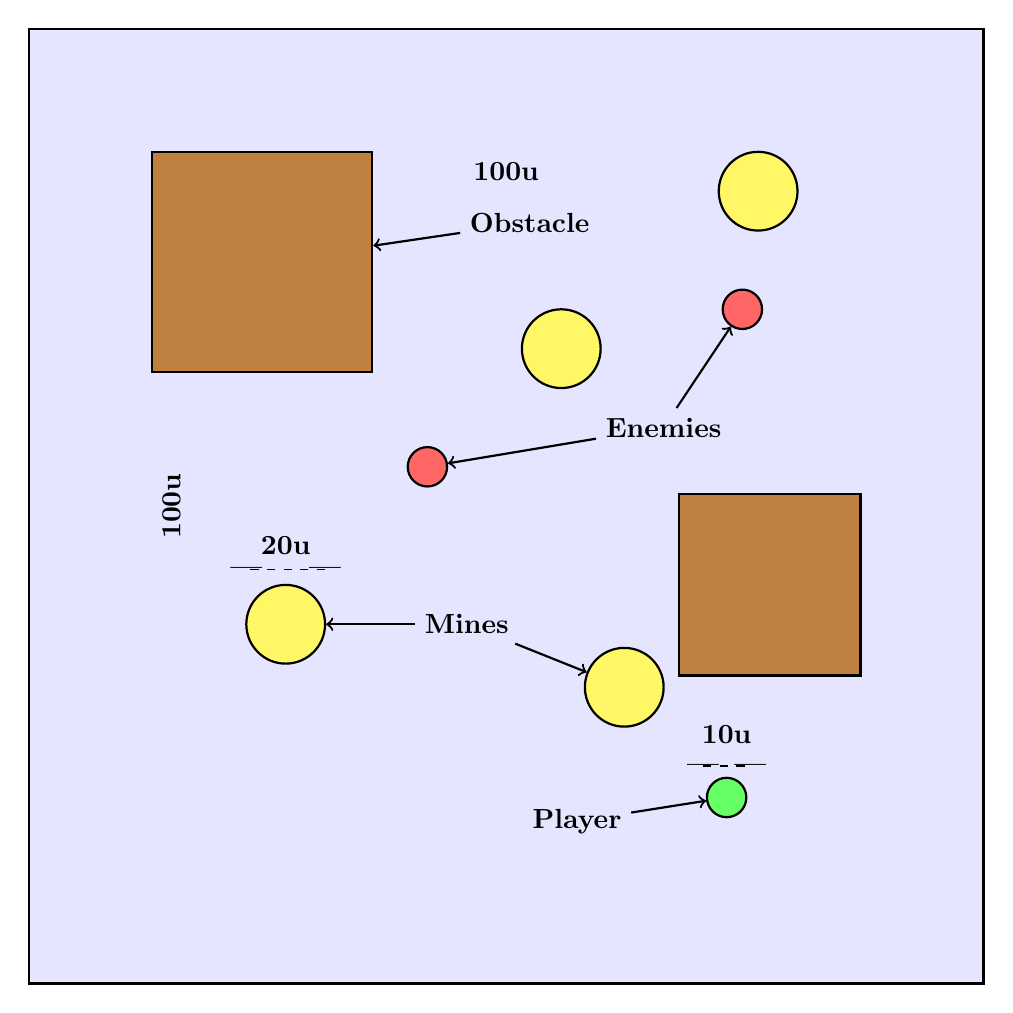
\begin{tikzpicture}[]
	\tikzstyle{sub}=[thick, draw, circle, align=center, minimum size = 0.5cm]					
	\tikzstyle{mine}=[thick, draw, circle, align=center, minimum size = 1cm, fill=yellow!60!white]					
	\tikzstyle{obstacle}=[thick, draw, rectangle, align=center, fill=brown]					
	\node[align=center, fill=blue!10!white, thick, draw, thick, rectangle, minimum height=\columnwidth, minimum width=\columnwidth](tarea)at (0,0) {};
	\node[](a1)at (0, 4.25) {\bf 100u};
	\node[rotate=90](a1)at (-4.25, 0) {\bf 100u};
	
	\node[obstacle, minimum size=2.8cm](obs1)at (-3.1, 3.1) {};
	\node[obstacle, minimum size=2.3cm](obs2)at (3.35, -1) {};
	\node[](tobs)at (0.3, 3.6) {\bf Obstacle};
	\draw[->, thick](tobs) -- (obs1);

	\node[fill=green!60!white, sub](player)at (2.8, -3.7) {};	
	\node[](tplayer)at (0.9, -4) {\bf Player};
	\draw[->, thick](tplayer) -- (player);
	\node[](a1)at (3.1, -3.3) {\bf |};
	\node[](a2)at (2.5, -3.3) {\bf |};
	\draw[-, dashed](2.5, -3.3) -- (3.1, -3.3);
	\node[](a2)at (2.8, -2.9) {\bf10u};
	
	\node[fill=red!60!white, sub](enemy1)at (-1, 0.5) {};	
	\node[fill=red!60!white, sub](enemy2)at (3, 2.5) {};
	\node[](tenemy)at (2, 1) {\bf Enemies};
	\draw[->, thick](tenemy) -- (enemy1);
	\draw[->, thick](tenemy) -- (enemy2);
	
	\node[mine](mine1)at (-2.8, -1.5) {};	
	\node[mine](mine2)at (1.5, -2.3) {};
	\node[mine](mine3)at (0.7, 2) {};
	\node[mine](mine4)at (3.2, 4) {};
	\node[](tmines)at (-0.5, -1.5) {\bf Mines};
	\draw[->, thick](tmines) -- (mine1);
	\draw[->, thick](tmines) -- (mine2);
	
	\node[](a1)at (-3.3, -0.8) {\bf |};
	\node[](a2)at (-2.3, -0.8) {\bf |};
	\draw[-, dashed](-2.3, -0.8) -- (-3.3, -0.8);
	\node[](a2)at (-2.8, -0.5) {\bf20u};	
	\end{tikzpicture}
\end{figure}
%
\vfill
%
At the start of the game, spread the player and enemy submarines as well as possible obstacles on the map.
In addition, determine the positions of the mines, but keep them secret until they are stepped on or detected by the sonar.
Before the game starts, the players can choose one of 3 difficulty levels, which determines the amount mines and enemy submarines, as well as the prize received for winning.
%
\\\\
%
\oftable{p{0.2\columnwidth} p{0.35\columnwidth} p{0.4\columnwidth}}
{\accf{Difficulty} & \accf{Enemies / Mines} & \accf{Prize}}
{
	Easy 	& 1 / 2 & Dark Matter \ofrow
	Medium	& 2 / 4 & Wet Floor Materia \ofrow
	Hard 	& 3 / 6 & Gold Hairpin \ofrow
}
%
\clearpage
%
%
%
%
%
%
%
%
%
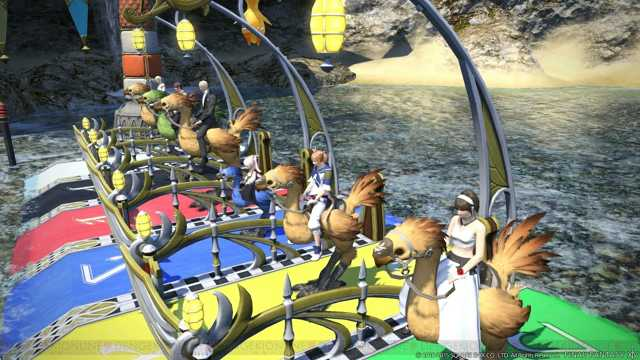
\includegraphics[width=\columnwidth]{./art/goldsaucer/chocoborace.jpg}
%
\vfill
%
\accf{Chocobo Racing} is a racing game with an entry fee of 2 GP per player.
Each player is a rider in the race and they can either choose one of the following Chocobos provided by the park or they can use a Chocobo that they own.
The GM adds and plays additional participants in the race until there are 5 competitors in total.
%
\\\\
%
\oftable{p{0.35\columnwidth} p{0.3\columnwidth} p{0.3\columnwidth}}
{\accf{Chocobo} & \accf{Stamina} & \accf{Agility}}
{
	Echo 	& 4 & 5 \ofrow
	Fives 	& 5 & 4 \ofrow
	Rex 	& 6 & 3 \ofrow
	Cody 	& 7 & 2 \ofrow
	Jesse   & 8 & 1 
}
%
\vfill
%
A race consists of multiple rounds and during a round, each participant performs a sprint check to determine which distance they can cover.
Participants continuously add up the results of all their checks as their total score and the first one to surpass 50 points wins the race.
The score of every participant should be announced at the end of each round to keep track of the current state of the race.
If multiple participants reach the finish line in the same round, the one with the highest score wins the race.
The sprint check performed on each turn is modified as follows:\ofrow
%
\ofbullet{%
	The result of each sprint check is reduced by the difference between the Chocobo's Stamina and its current fatigue. 
	Everyone starts with 0 fatigue and gains 1 fatigue at the end of each round.
	For example, if a Chocobo has a fatigue of 10 and a Stamina of 8, the result of their check would be reduced by 2, but if  it had 10 or more Stamina it would receive no penalty.
	This reduction cannot cause the result of a sprint to drop below 0.
}
\ofbullet{%
	Before each check, a participant can decide to perform a dash action.
	In this case, they gain Advantage on the sprint check, but also an additional point of fatigue.
	Within a race, you can dash only a maximum amount of times equal to the Chocobo's Agility.
}
\ofbullet{%
	Characters who are particularly good at handling Chocobos gain Advantage on all sprint checks.
}
%
\\\\
%
When the race is finished, the winner rolls 1d and receives a prize based on the result.
%
\newpage
%
\oftable{p{0.4\columnwidth} p{0.7\columnwidth}}
{\accf{Result} & \accf{Prize}}
{
	1 & 10 GP \ofrow
	2 & Phoenix Down \ofrow
	3 & Signal Materia \ofrow
	4 & Elixir \ofrow
	5 & Angel Materia \ofrow
	6 & Hermes Boots
}
%
\\\\
%
%
%
%
%
%
%
%
%
\begin{center} 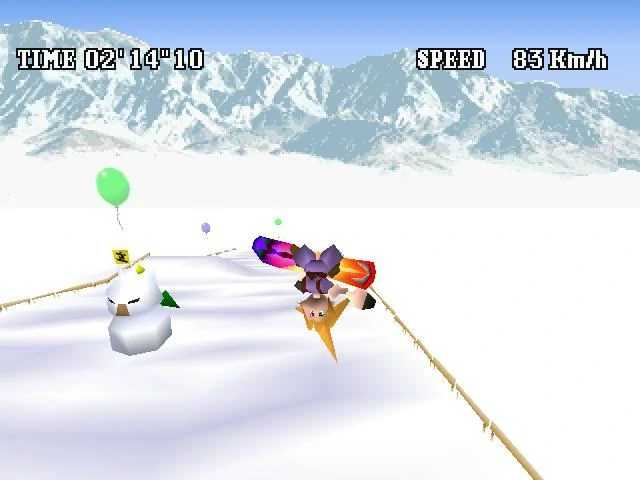
\includegraphics[width=\columnwidth]{./art/goldsaucer/snowgame.jpg} \end{center}
\accf{Snow Game} is a snowboarding game that costs 1 GP to play per player.
The game can be played by multiple players who race down a ski run trying to reach a high score.
This score starts at 0, collecting balloons increases it, while hitting obstacles reduces it, so the score can become negative.
The course has 3 lanes: left, center and right and the players start on the center lane, going down the ski run back to back.
The game plays out over 8 rounds and at the start of each round, the GM rolls 3d, one die after the other, to determine the objects on the 3 lanes in front of the players from left to right.
The table below shows the possible objects based on the die results and their effects that occur when a players collide with them.
%
\\\\
%
\oftable{p{0.3\columnwidth} p{0.35\columnwidth} p{0.3\columnwidth}}
{\accf{Result} & \accf{Object} & \accf{Effect}}
{
	1 - 2 & Nothing & -- \ofrow
	3 & Snowman & - 1 point\ofrow
	4 & Rock & - 2 points \ofrow
	5 & Red Balloons & + 1 point\ofrow
	6 & Blue Balloons & + 2 points \ofrow
}
%
\\\\
%\clearpage
%
After learning about the objects in front of them, each player can decide between 1 of 3 actions:\ofrow
\ofbullet{\accf{Move one lane to the left or right:} make a DC~6 check, if you succeed you successfully change one lane, otherwise you stay in your current one.} 
\ofbullet{\accf{Move two lanes to the left or right:} make a DC~8 check, if you succeed you successfully change two lanes, otherwise you stay in your current one.} 
\ofbullet{\accf{Jump:} make a DC~8 check. If you succeed, you avoid the object in front of you and you gain 1 point. If you fail, you collide with the object in front of you and you additionally lose 1 point. You can take this action even if there are not objects in front of you.} \ofrow
Characters with particularly good coordination or experience with snowboards gain Advantage on these checks.
After all actions have been taken, check which lane each player ends up in and whether they collide with any objects to adjust the scores accordingly before the next round starts.
At the end of the 8th round, all players reaches the finish line and depending on their score each player receives one of the following prices.
%
\\\\
%
\oftable{p{0.4\columnwidth} p{0.7\columnwidth}}
{\accf{Score} & \accf{Prize}}
{
	< 4 & Participation Trophy \ofrow
	4 - 5 & X-Potion \ofrow
	6 - 7 & Safety Bit \ofrow
	8 - 9 & HP Plus \ofrow
	> 9 & 50 GP \ofrow
}
%
%
\ofpar
%
%
%
%
%
%
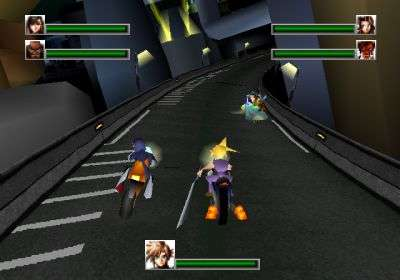
\includegraphics[width=\columnwidth]{./art/goldsaucer/gbike.jpg}
\\\\
\accf{G-Bike} is a biking game where the players are chased by hostile bikers on a highway and have to fight them off to escape.
The game can be played by multiple players with an entry fee of 1 GP per player.
The highway has 4 lanes and the focus is always put on 3 rows, so there are 12 total positions where bikers and obstacles can be positioned at a given time.
The illustration below shows how the map might look like during the game.
%
%\newpage
%
\begin{figure}[h!]
	\centering
	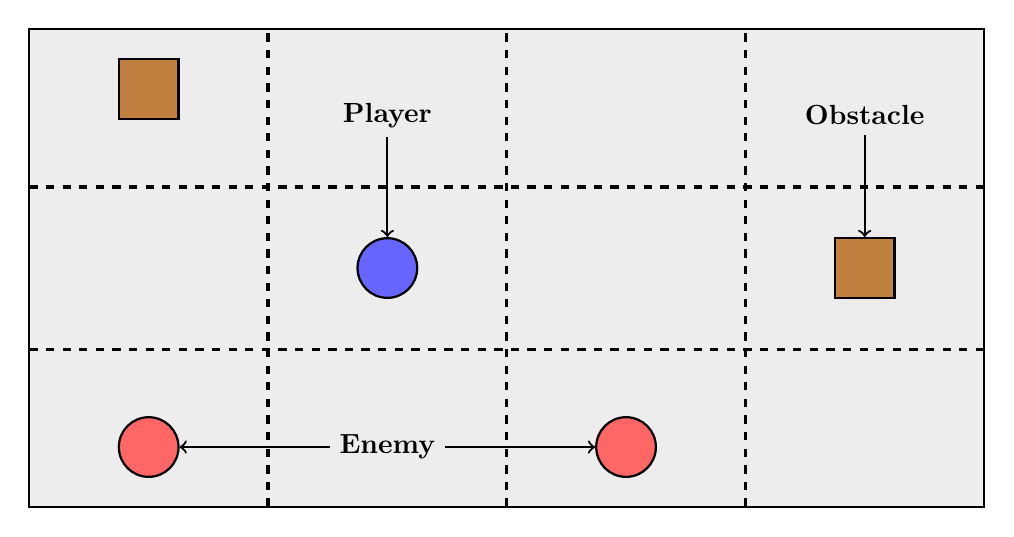
\begin{tikzpicture}[]
	\tikzstyle{biker}=[thick, draw, circle, align=center, minimum size = 0.5*0.125\columnwidth]					
	\tikzstyle{obstacle}=[thick, draw, rectangle, align=center, fill=brown, minimum size=0.5*0.125\columnwidth]					
	
	\node[align=center, thick, draw, thick, rectangle, minimum height=0.5\columnwidth, minimum width=\columnwidth, fill=black!7!white](tarea)at (0,0) {};		
	\draw[very thick, -, dashed](-0.25\columnwidth, -0.25\columnwidth) -- (-0.25\columnwidth, 0.25\columnwidth);
	\draw[very thick, -, dashed](0, -0.25\columnwidth) -- (0, 0.25\columnwidth);
	\draw[very thick, -, dashed](0.25\columnwidth, -0.25\columnwidth) -- (0.25\columnwidth, 0.25\columnwidth);
	\draw[very thick, -, dashed](-0.5\columnwidth, 0.5*-0.17\columnwidth) -- (0.5\columnwidth, 0.5*-0.17\columnwidth);
	\draw[very thick, -, dashed](-0.5\columnwidth, 0.5*0.17\columnwidth) -- (0.5\columnwidth, 0.5*0.17\columnwidth);
	
	\node[fill=red!60!white, biker](b1)at (-0.375\columnwidth, 0.5*-0.375\columnwidth) {};
	\node[fill=red!60!white, biker](b2)at (0.125\columnwidth, 0.5*-0.375\columnwidth) {};
	\node[fill=blue!60!white, biker](b3)at (-0.125\columnwidth, 0) {};
	\node[obstacle](obs1)at (0.375\columnwidth, 0) {};
	\node[obstacle](obs2)at (-0.375\columnwidth, 0.5*0.375\columnwidth) {};
	
	\node[](tobs)at (0.375\columnwidth, 0.16\columnwidth) {\bf Obstacle};
	\draw[->, thick](tobs) -- (obs1);
	\node[](tplayer)at (-0.125\columnwidth, 0.16\columnwidth) {\bf Player};
	\draw[->, thick](tplayer) -- (b3);
	\node[](tenemy)at (-0.125\columnwidth, 0.5*-0.375\columnwidth) {\bf Enemy};
	\draw[->, thick](tenemy) -- (b1);
	\draw[->, thick](tenemy) -- (b2);
	\end{tikzpicture}
\end{figure}
%
\newpage
%
The game plays out over 8 rounds and during each round, first all players take one turn and then all hostile bikers.
Player bikers start with 3 HP and enemy bikers start with 1 HP, when a biker is reduced to 0 HP, he is removed from the game.
During a turn, each biker may make a movement and take one Attack action:
\vfill
\ofbullet{\accf{Movement:} move either one lane to the left / right or one row to the front / back if that position is not occupied by an obstacle or another biker. Alternatively, you can try to activate the bike turbo. In this case, make a DC~8 check, if you succeed you can make two movements on this turn, if you fail, you cannot move at all. Characters with particularly good vehicle handling receive Advantage on this check}\ofpar
\ofbullet{\accf{Melee Attack:} make a DC~6 check. If you succeed, a biker who is 1 movement away from you suffers 1 HP damage.}\ofpar
\ofbullet{\accf{Ranged Attack:} make a DC~8 check. If you succeed, a biker who is 2 or less movements away from you, suffers 1 HP damage.}
%
\vfill
%
At the start of each round, roll 1d for every player that is still in the game.
Based on the results, place the following items in any open position of your choice: 1-2:nothing, 3:red biker,  4:blue biker, 5-6:obstacle.
However, do not place any more hostile bikers if there are already as many of them in the game as players.
Red and blue bikers are controlled by the GM and follow the same rules as players, but red bikers can only perform ranged attacks while blue bikers can only perform melee attacks.
Obstacles all follow the same rules and the GM is free to choose their appearance, they could for example be roadblocks or other vehicles.
Whenever a player biker ends his turn with an obstacle in the same lane in front of him, he has to make a DC~8 check, if he succeeds he jumps over the obstacle and if not, he suffers 1 HP damage.
Enemy bikers evade all obstacles automatically.
At the end of each round, all bikers stay in their positions and all obstacles disappear as they are left behind the current field of focus.
Every player biker who survives until the end of the 8th round wins a prize.
Each winner rolls 1d and depending on the result, he receives one of the following prizes.
%
\vfill
%
\oftable{p{0.4\columnwidth} p{0.5\columnwidth}}
{\accf{Result} & \accf{Prize}}
{
	1 	 & Item Holder \ofrow
	2    & 5 GP \ofrow		
	3    & Turbo Ether \ofrow
	4    & Phoenix Down \ofrow
	5    & Alert Materia \ofrow    
	6    & Bomb Materia
}
%
\clearpage
%
%
%
%
%
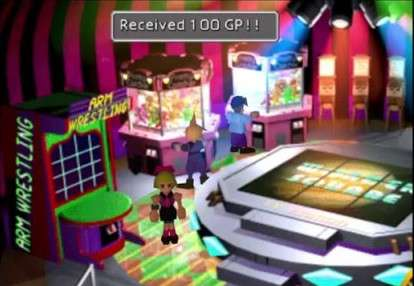
\includegraphics[width=\columnwidth]{./art/goldsaucer/proxycatcher.jpg}
%
\vfill
%
\accf{Proxy Catcher} is a crane game that costs 4 GP to play.
The game is played by a single player who uses the controls of the machine to navigate a crane and potentially pick a valuable prize from a pile.
The player only has one chance to lower the crane and grab something.
To do so, the player makes a check and receives a prize based on the result as listed in the table below.
However, the game is rigged as the crane has a fixed chance of properly grabbing something.
Players can perform a DC~8 check to understand that the player skill has barely any influence on the odds of success.
%
\vfill
%
\oftable{p{0.5\columnwidth} p{0.5\columnwidth}}
{\accf{Result} & \accf{Prize}}
{
	2 - 5 & Nothing \ofrow
	6 - 7 & Potion \ofrow
	8     & 5 GP \ofrow		
	9     & Ether \ofrow
	10    & Phoenix Down \ofrow
	11    & 20 GP \ofrow    
	12    & Counter Materia
}
\vfill
%
{
\begin{center}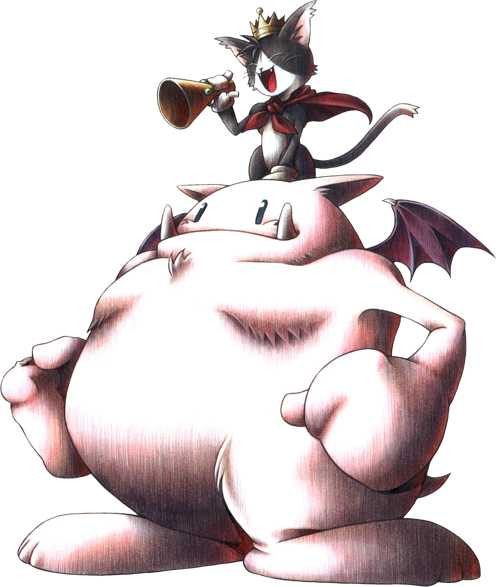
\includegraphics[width=0.7\columnwidth]{./art/goldsaucer/caitsith.jpg}\end{center}
%
%
%
%
\newpage
%
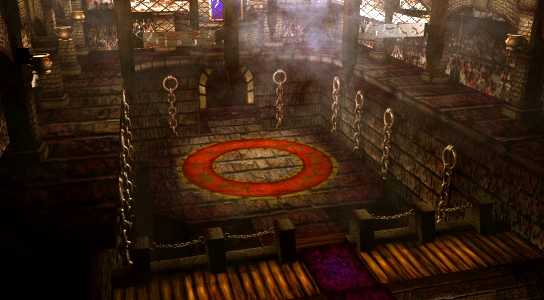
\includegraphics[width=\columnwidth]{./art/goldsaucer/arena.jpg}
%
\vfill
%
The \accf{Colosseum} is a battle arena that costs 1 GP per player to participate in.
All players that want to participate, fight up to 7 groups of monsters together as a party, one after another, on a 10u by 10u battlefield with walls on all 4 sides.
After the party defeats one group, roll 1d and depending on the result, they receive an additional handicap in each subsequent fight.
If you roll the same number twice, roll again until you get a handicap that is not active yet.
The list below shows the 6 possible handicaps, so by time the party reaches the 7th round, all of them will be active.
%
\vfill
%
\oftable{p{0.15\columnwidth} p{0.75\columnwidth}}
{\accf{Result} & \accf{Handicap}}
{
	1 & You can no longer equip Materia. \ofrow
	2 & You can no longer use Items.  \ofrow
	3 & You can no longer equip Accessories. \ofrow
	4 & You can no longer equip Armor.  \ofrow
	5 & You can no longer use Limit Breaks. \ofrow
	6 & You suffer Zombie until you leave the Colosseum (cannot be removed). \ofrow
}
%
\vfill
%
After defeating a group, everyone in the party can take an additional turn before the next fight starts.
At that point, they can also decide to forfeit and collect a prize depending on how many rounds they have completed.
If the entire party is defeated within a round, they do not receive any prize.
In any case, the party fully recovers their HP and MP after leaving the Colosseum.  
The list below shows the possible prizes depending on how many rounds were completed.
The following page shows the 7 types of monsters encountered from the 1st to the 7th round.
At the start of each round, place as many of the current round's monster type on the battlefield as there are players.
%
\vfill
%
\oftable{p{0.4\columnwidth} p{0.75\columnwidth}}
{\accf{Round} & \accf{Prize}}
{
	1 & Potion \ofrow
	2 & Phoenix Down \ofrow
	3 & 10 GP \ofrow
	4 & Lure Materia  \ofrow
	5 & Blaze Materia \ofrow
	6 & Protect Bangle \ofrow
	7 & Genji Gloves \ofrow
}
%
\clearpage
%
\ofmonster{Python (Round 1)}{3}{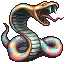
\includegraphics[width=0.2\columnwidth]{./art/goldsaucer/python.jpg}}
{
	HP: & \hfill 24 & MP: & \hfill 18\\
	STR: & \hfill 3 & DEF: & \hfill 1 \\
	MAG: & \hfill 0 & RES: & \hfill 3 \\
	AGI: & \hfill 3 & Size: & \hfill M\\
}
{\accf{Bite}: 1d DMG \hfill \accf{Immune:}\poison \hfill \accf{Weak:}\earth}
{	
	\mtech{Entangle}{6}{0r}{Single}{3u}{The target makes a DC 8 check and suffers 2d damage and Immobile for 1 round upon failure.}{\immobile}		
}
%
\vfill
%
\ofmonster{Hecteyes (Round 2)}{4}{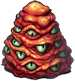
\includegraphics[width=0.2\columnwidth]{./art/goldsaucer/hecteyes.jpg}}
{
	HP: & \hfill 32 & MP: & \hfill 50\\
	STR: & \hfill 1 & DEF: & \hfill 2 \\
	MAG: & \hfill 6 & RES: & \hfill 8 \\
	AGI: & \hfill 2 & Size: & \hfill M\\
}
{\accf{Tackle}: 2d DMG \hfill \accf{Immune:}\sleep \hfill \accf{Weak:}\lightning}
{	
	\mspell{Blind}{6}{1r}{Single}{3u}{The target makes a DC 8 check and suffers Blind for 3 round upon failure.}{\blind}		
	\mspell{Thunder}{4}{1r}{Single}{3u}{You deal 2d lightning damage to the target.}{\ice}		
}
%
\vfill
%
\ofmonster{Mantis (Round 3)}{5}{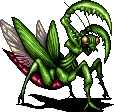
\includegraphics[width=0.23\columnwidth]{./art/goldsaucer/mantis.jpg}}
{
	HP: & \hfill 46 & MP: & \hfill 30\\
	STR: & \hfill 4 & DEF: & \hfill 2 \\
	MAG: & \hfill 0 & RES: & \hfill 2 \\
	AGI: & \hfill 3 & Size: & \hfill M\\
}
{\accf{Cut}: 2d DMG \hfill \accf{Immune:}\immobile \hfill \accf{Weak:}\fire}
{	
	\mtech{Metal Cutter}{4}{0r}{Single}{Weapon}{Make an Attack against the target. If you succeed, the damage dealt ignores the target's DEF.}{}		
	\mpassive{Leap}{When moving you can jump over enemies and obstacles up to a height of 2u, instead of having to walk around them.}	
}
%
\vfill
%
\ofmonster{Griffon (Round 4)}{6}{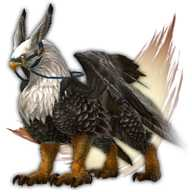
\includegraphics[width=0.23\columnwidth]{./art/goldsaucer/griffon.jpg}}
{
	HP: & \hfill 67 & MP: & \hfill 50\\
	STR: & \hfill 6 & DEF: & \hfill 3 \\
	MAG: & \hfill 0 & RES: & \hfill 5 \\
	AGI: & \hfill 3 & Size: & \hfill M\\
}
{\accf{Claw}: 2d DMG \hfill \accf{Immune:}\immobile\blind \hfill \accf{Resilient:}\wind}
{	
	\mtech{Feather Shot}{6}{0r}{Single}{4u}{The target suffers 3d wind damage.}{\wind}		
	\mpassive{Peck}{Whenever you successfully Attack a target he makes a DC 7 check and suffers Blind for 3 rounds upon failure.}
}
%
\newpage
%
\ofmonster{Big Horn (Round 5)}{7}{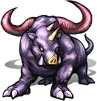
\includegraphics[width=0.23\columnwidth]{./art/goldsaucer/bighorn.jpg}}
{
	HP: & \hfill 90 & MP: & \hfill 80\\
	STR: & \hfill 7 & DEF: & \hfill 5 \\
	MAG: & \hfill 0 & RES: & \hfill 5 \\
	AGI: & \hfill 2 & Size: & \hfill L\\
}
{\accf{Tackle}: 3d DMG \hfill \accf{Immune:}\poison \hfill \accf{Resilient:}\fire}
{	
	\mtech{Charge}{8}{1r}{Single}{10u}{Dash towards the target and deal 3d damage to him. In addition, the target is knocked back by 3u and if he hits a wall, he suffers an additional 3d damage.}{}		
	\mreaction{Kickback}{Whenever you suffer damage from an enemy within 1u, you can deal 10 physical damage to him and knock him back by 2u.}
}
%
\vfill
%
\ofmonster{Golem (Round 6)}{8}{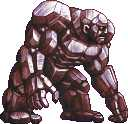
\includegraphics[width=0.23\columnwidth]{./art/goldsaucer/golem.jpg}}
{
	HP: & \hfill 130 & MP: & \hfill 100\\
	STR: & \hfill 9 & DEF: & \hfill 8 \\
	MAG: & \hfill 0 & RES: & \hfill 6 \\
	AGI: & \hfill 2 & Size: & \hfill L\\
}
{\accf{Fist}: 3d DMG \hfill \accf{Immune:}\poison\sleep\ \hfill \accf{Resilient:}\earth}
{	
	\mspell{Quake}{20}{1r}{3u}{7u}{Deal 6d earth damage to everyone in the target area.}{\earth}
	\mtech{Earth Wall}{12}{0r}{3u (line)}{3u}{You create a 3u tall and wide wall of earth that blocks the path. The wall breaks down after 3 rounds or upon suffering a total of 15 damage.}{}
}
%
\vfill
%
\ofmonster{Dark Dragon (Rnd 7)}{9}{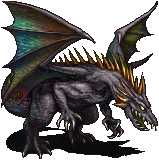
\includegraphics[width=0.24\columnwidth]{./art/goldsaucer/blackdragon.jpg}}
{
	HP: & \hfill 200 & MP: & \hfill 180 \\
	STR: & \hfill 10 & DEF: & \hfill 7 \\
	MAG: & \hfill 9 & RES: & \hfill 8 \\
	AGI: & \hfill 3 & Size: & \hfill L\\
}
{\accf{Bite}: 3d DMG \hfill \accf{Resilient}:\fire\ice\dark \\ \accf{Immune}: All Status Effects}
{
	\mtech{Obliterating Breath}{16}{0r}{3u (front)}{3u}{Everyone in the target area makes a DC 8 check and suffers 4d damage as well as Poison and Blind for 3 rounds upon failure.}{\poison \blind}{}
	\mspell{Dark Flare}{30}{2r}{Single}{5u}{You deal 6d+20 dark damage to the target.}{\dark}
	\mpassive{Tail Whip}{Whenever you Attack, you can choose to target all enemies within 1u at once.}	
}	
%
\clearpage